\documentclass[10pt]{article}
\usepackage[margin=0.73in]{geometry}
\usepackage{amsmath,amssymb,graphicx,booktabs,xcolor,hyperref}
\definecolor{ink}{HTML}{253C59}
\hypersetup{colorlinks=true,urlcolor=ink,linkcolor=ink}
\setlength{\parindent}{0pt}\setlength{\parskip}{6pt}
\begin{document}
{\Large\bfseries\color{ink} Guarded section coefficient elimination}\par
{\small 23 November 2026 \quad Local correctness controls; degree and fill tradeoff}

\textbf{Implemented block.} A separate Rust compiler retains every original
six-member point variable and equation. Its regular chart requires finite
$R=(r,s)$, $s\ne0$, six distinct $x_i$ and $x_i\ne r$, with 21 explicit inverse
guards. The normalized section has $c_4=1$; its rows are
\[
[(x-r),\;x(x-r),\;y(x-r),\;x^2(x-r),\;xy(x-r),\;s+y].
\]
The augmented reference keeps five coefficient unknowns and all six rows.
Each of six pivot choices replaces them with one inverse $t$, guarded by
$tD=1$, and the remaining cleared row. Reconstruct $c_i=tN_i$. All five
selected-row sparse identities $AN-bD$ must cancel at compilation. The full
augmented reference remains available; a zero pivot is not absence.
Classical Cramer/Schur elimination is not novel. [pcc:PCC-20261123-d83c36]

\textbf{Fixed controls.} Corrected v2 completes 12 supplied fixtures: 10 admitted,
two identity-target exclusions, 60 nonzero-pivot lift/projections. Reconstructed
coefficients match; original/inverse/coefficient and canonical/length controls
refuse corruption. Independent numeric section, raw-$R$ and original indexed
image-$Q$ group replay pass on admitted controls. Five release unit tests,
fmt and strict all-target Clippy pass locally. Rank-deficient/zero-minor and
inconsistent-residual matrix controls are included. No backend invocation or
unknown root discovery. [pcc:PCC-20261123-d83c36]

V/E/T denote variables, equations and terms.
\begin{center}
\begin{tabular}{lll}
\toprule Fixed chart 0 & Augmented V/E/T/degree & Eliminated V/E/T/degree\\\midrule
Toy support 1 &353/384/1274/4&349/380/6963/12\\
$q=213156431,\ k=20633$ &1085/1116/3458/4&1081/1112/9147/12\\\bottomrule
\end{tabular}
\end{center}
\textbf{Observed tradeoff.} Four net variables removed; degree 4 becomes 12 and
sparse fill grows. The direct original point system is still smaller in
variables: 327 toy, 1059 actual-k20633. New guards/sector constraints restrict the
domain. These are representation counts, not a solver-cost ranking or attack
exponent. Each listed chart records 105276 sparse product-pair reservations,
including identity checking; many original construction, allocation, parsing,
field/bit and replay costs are unpriced. [pcc:PCC-20261123-d83c36]

\textbf{Scope.} Identity target, +/-R members, repeated x/aliases/jets and
unresolved rank strata are outside this admitted chart. Raw-$R$ versus
image-$Q$ completeness is still open. No full family or solver bound follows
from sixty fixed projections. [pcc:unverified]

\newpage
{\large\bfseries\color{ink} Evidence, publication and the missing search rule}
\begin{center}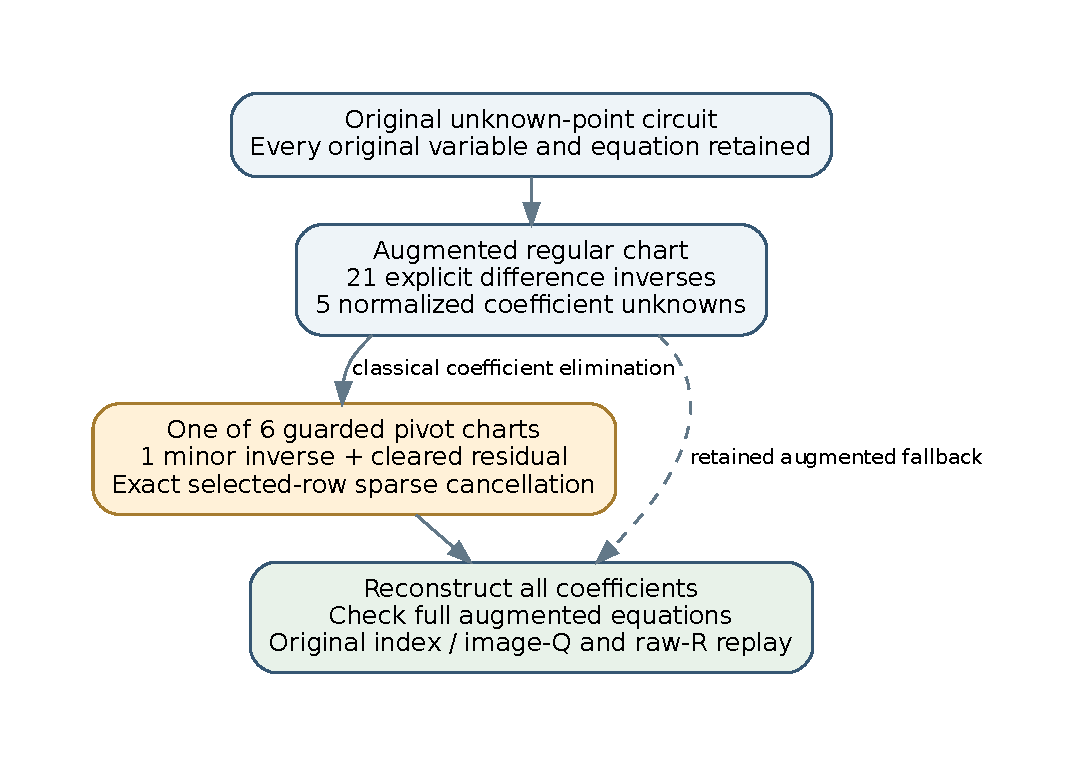
\includegraphics[width=0.9\linewidth,height=2.6in,keepaspectratio]{diagram.pdf}\end{center}

\textbf{First-call failure preserved.} V1 stopped after eight completed
fixtures: the harness propagated a correctly unsupported identity-target
refusal. Its source, binary and full partial run remain frozen. V2 changes
only that classification and records the two excluded targets. Algebra,
fixtures, caps and admitted acceptance are unchanged. Each version has 103
source inputs in four constituents: unchanged 95 plus new 8. Six compiled
source hashes and the old fixture hash match. Separate write-once build/
precall/postcall and binary pre/post checks; no source edits/tests after
qualification. [pcc:PCC-20261123-d83c36]

\textbf{Raw publication incomplete.} Full polynomial/witness streams remain
in lossless 178488-byte and 272444-byte archives, both selected by actual
artifact policy. They are retained locally untracked, with exact inventories
and readback. Maintained upload refused for unavailable credentials; no real
receipt or store pointer exists. Statement d83c36 binds source/summary/raw
inventory metadata; it is unsigned/not\_covered. No evidence substitution,
policy exemption, credential export or remote deletion.

\textbf{Next exponent-facing object.} Derive a non-enumerating section
selection/elimination rule with explicit $q,k$ dependence. A supplied-point
interpolation and logarithmic-depth quotient circuits provide no solving-degree
bound. Preserve labels/ranges, original projection and every guard, then charge
full cold work and useful yield. Full chart/sector proofs, independent relation
rank, private selection, memory/indexing/setup and recovery remain open. Do not
scale the expanded minors or raise generic caps based only on four fewer
variables. No paid worker or campaign is scheduled. [pcc:unverified]

\textbf{Sources.} Original section operator, compact spectrum compiler and
direct point comparator; native metadata statement PCC-20261123-d83c36.\par
Source identity: SOURCE\_QUALIFICATION\_V2.json.\par
Results: RESULTS\_V2.json; raw inventories in native-v1 and native-v2.\par
Cheng, \href{https://arxiv.org/pdf/cs/0507026}{Hard Problems of Algebraic Geometry Codes},
\S2/Theorem1; Snowden, \href{https://websites.umich.edu/asnowden/teaching/2013/679/L02.html}{Math679 lecture2}.
These supply the classical section/subset-sum context, not this family's
efficient root search. KB unavailable; no novelty or new Lean/compiler/group
theorem claimed. Existing immutable-record, old artifact and journal integration
obligations remain open; all earlier source/evidence/criteria are unchanged.
\end{document}
